\chapter{PCB Design and Schematics}


\section{ECG Shield PCB for AD8232 and Arduino Pro Mini}
\label{ecgshieldpcb}

\begin{figure}[H]
	\centering
	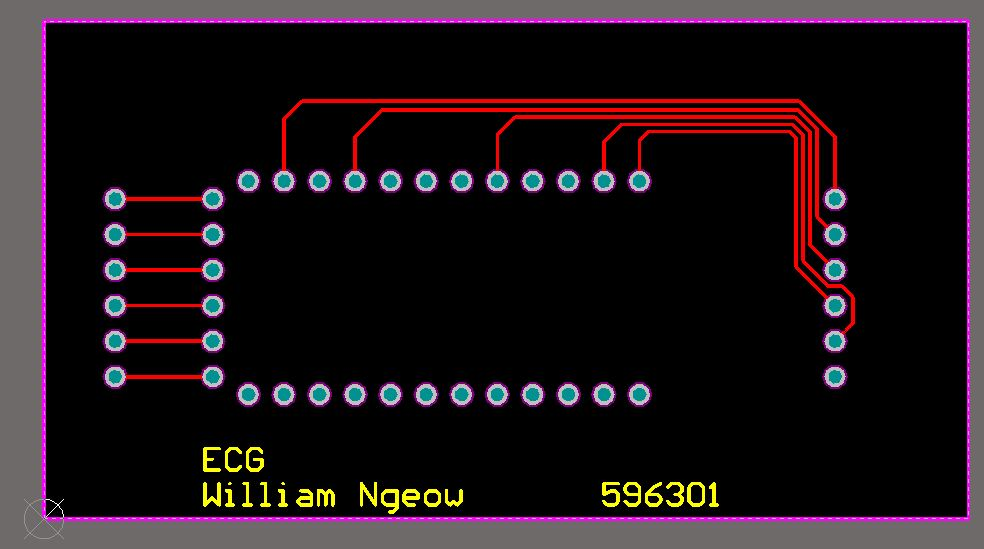
\includegraphics[width=0.8\linewidth]{ecgshield.jpg}
	\caption{ECG Shield PCB for AD8232 and Arduino Pro Mini}
\end{figure}

\section{Thermistor in Phase Shift Oscillator Configuration Schematic and PCB}

\begin{figure}[H]
	\centering
	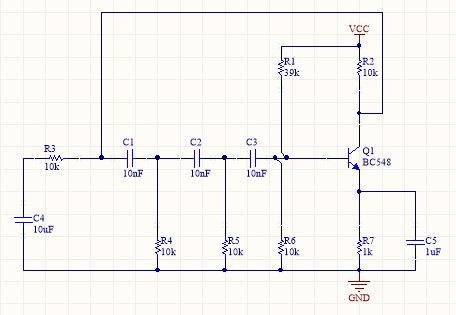
\includegraphics[width=0.7\linewidth]{psoschematic.jpg}
	\caption{Thermistor in Phase Shift Oscillator Configuration Schematic}
\end{figure}

\begin{figure}[H]
	\centering
	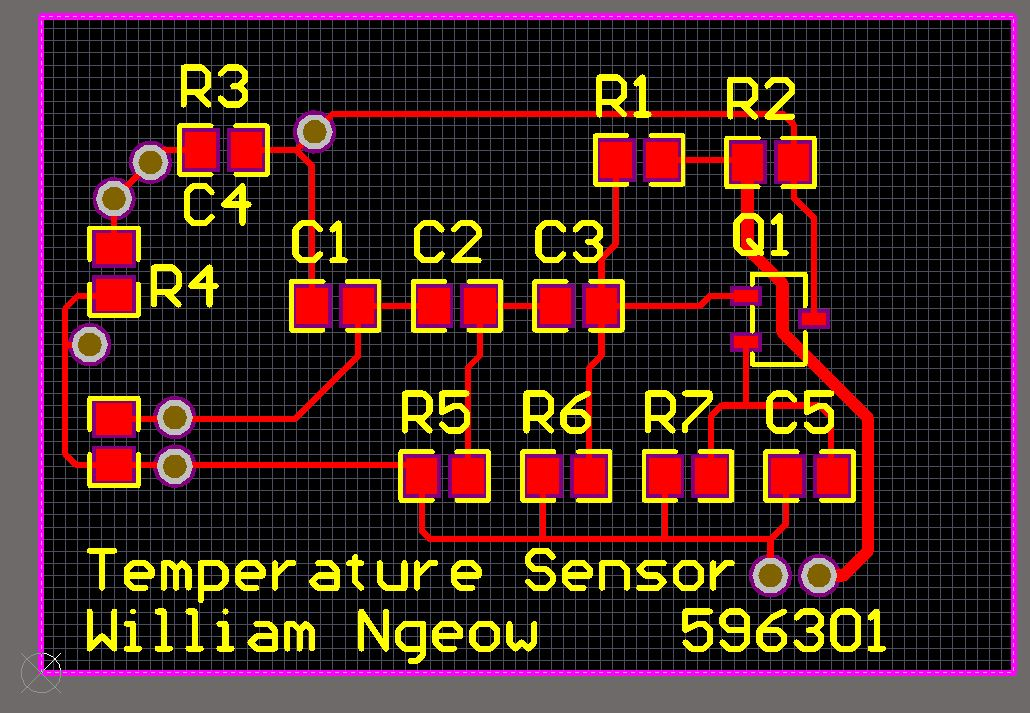
\includegraphics[width=0.8\linewidth]{psopcbnognd.jpg}
	\caption{Thermistor in Phase Shift Oscillator Configuration PCB}
\end{figure}

\section{AD8232 Heart Rate Monitor SparkFun Implementation}

\begin{figure}[H]
	\centering
	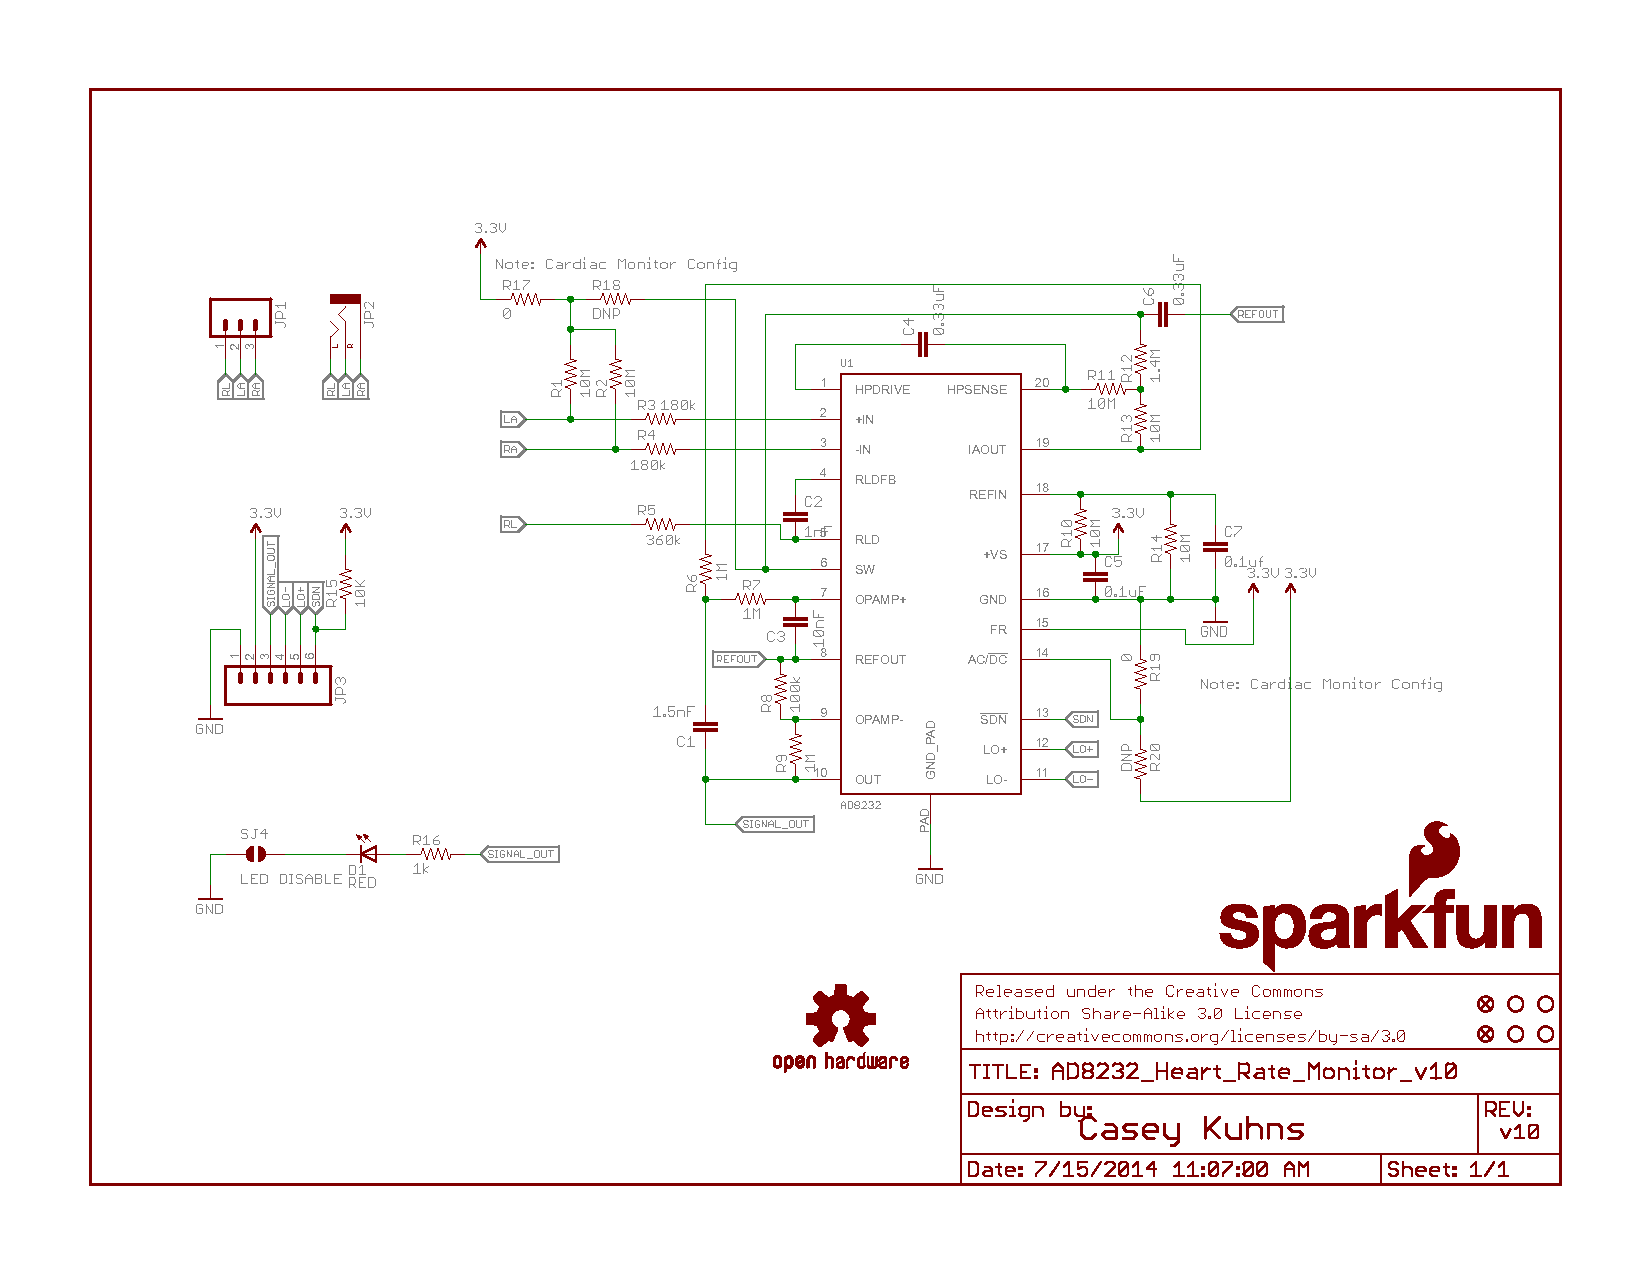
\includegraphics[width=1.05\linewidth]{AD8232_Heart_Rate_Monitor_v10.pdf}
	\caption{AD8232 SparkFun Implementation Schematic Diagram \cite{ad8232sfschematic}}
	\label{ad8232sfschematic}
\end{figure}

Further details of the design can be found at \\ https://github.com/sparkfun/AD8232\_Heart\_Rate\_Monitor.

\section{Raspberry Pi 3 Model B}

\begin{figure}[H]
	\centering
	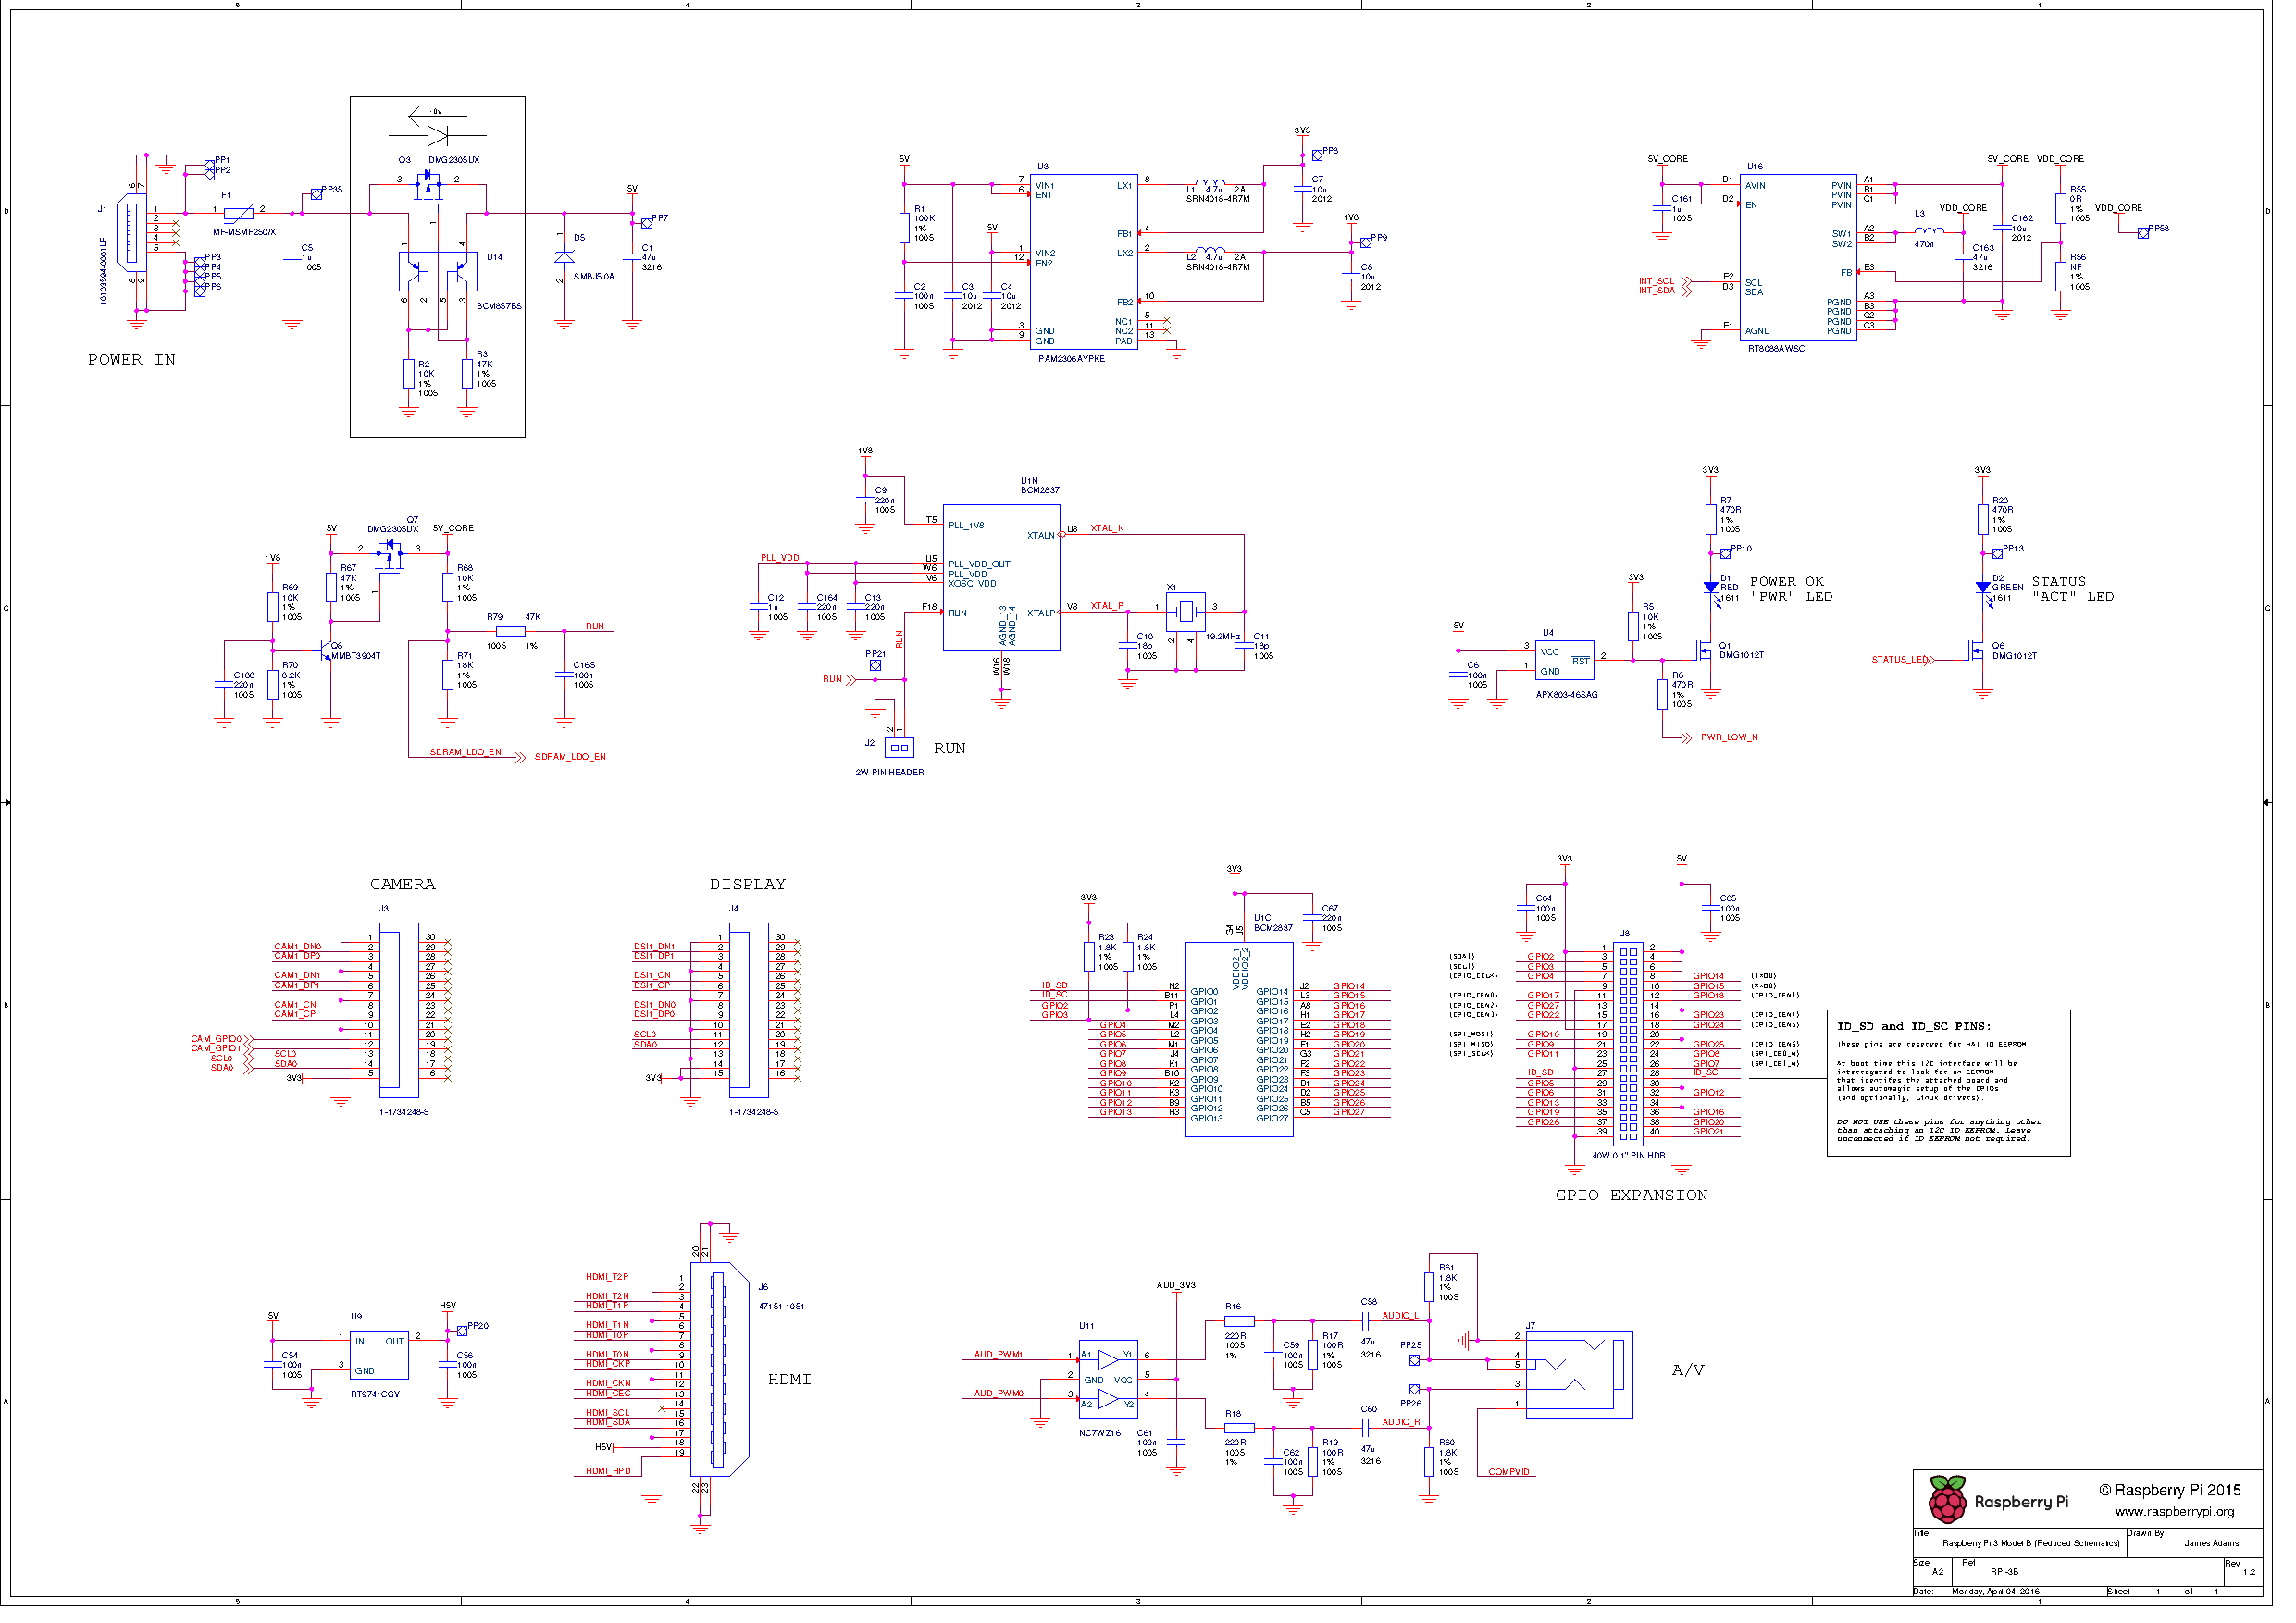
\includegraphics[width=1.25\linewidth,angle=90,origin=c]{RPI-3B.pdf}
	\caption{Raspberry Pi 3 Model B Schematic Diagram \cite{rpi3hardware}}
	\label{rpi3bschematic}
\end{figure}

Further details of the design can be found at \\ https://www.raspberrypi.org/documentation/hardware/raspberrypi/schematics/RPI-3B-V1\_2-SCHEMATIC-REDUCED.pdf.




\section{Transmitter Schematics for PPG}

\begin{figure}[H]
	\centering
	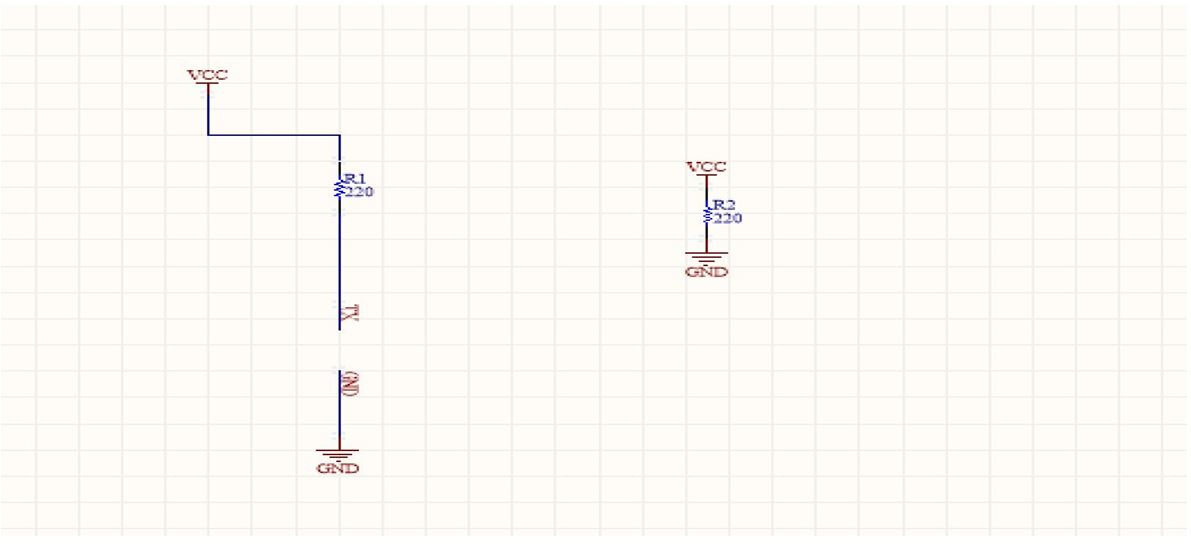
\includegraphics[width=\linewidth]{georgepic14.jpg}
	\caption{Transmitter Schematics for PPG}
\end{figure}

\section{Transmitter PCB for PPG}

\begin{figure}[H]
	\centering
	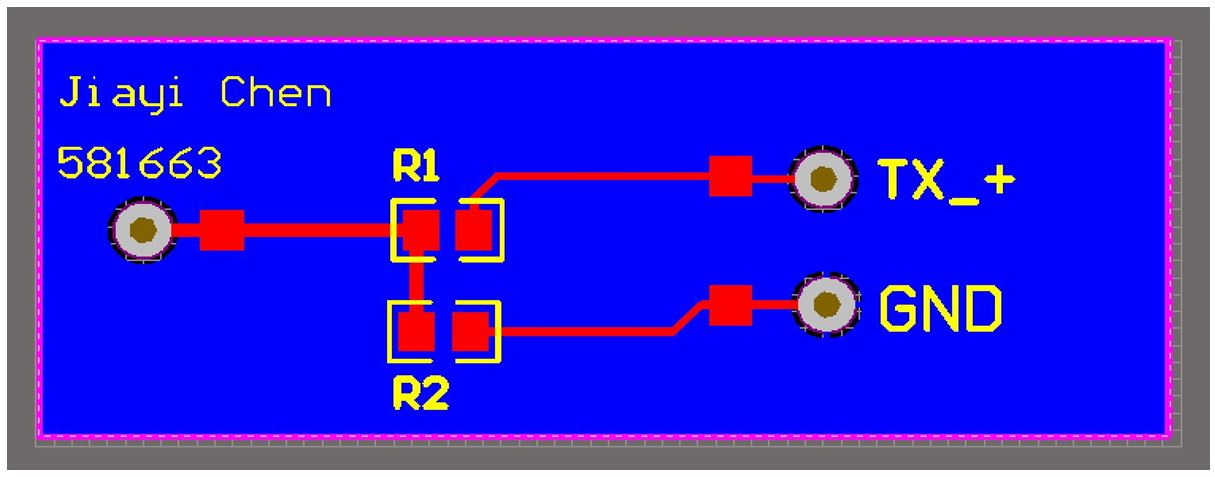
\includegraphics[width=\linewidth]{georgepic15.jpg}
	\caption{Transmitter PCB for PPG}
\end{figure}

\section{Receiver Schematics for PPG}

\begin{figure}[H]
	\centering
	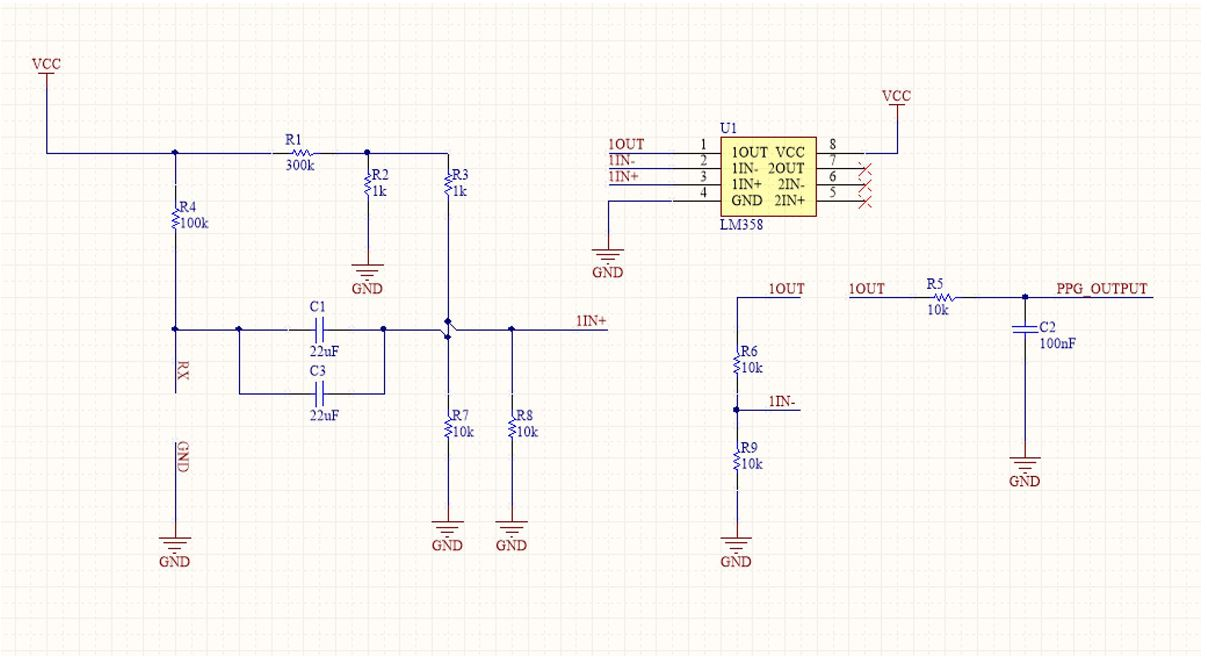
\includegraphics[width=\linewidth]{georgepic16.jpg}
	\caption{Receiver Schematics for PPG}
\end{figure}

\section{Receiver PCB for PPG}

\begin{figure}[H]
	\centering
	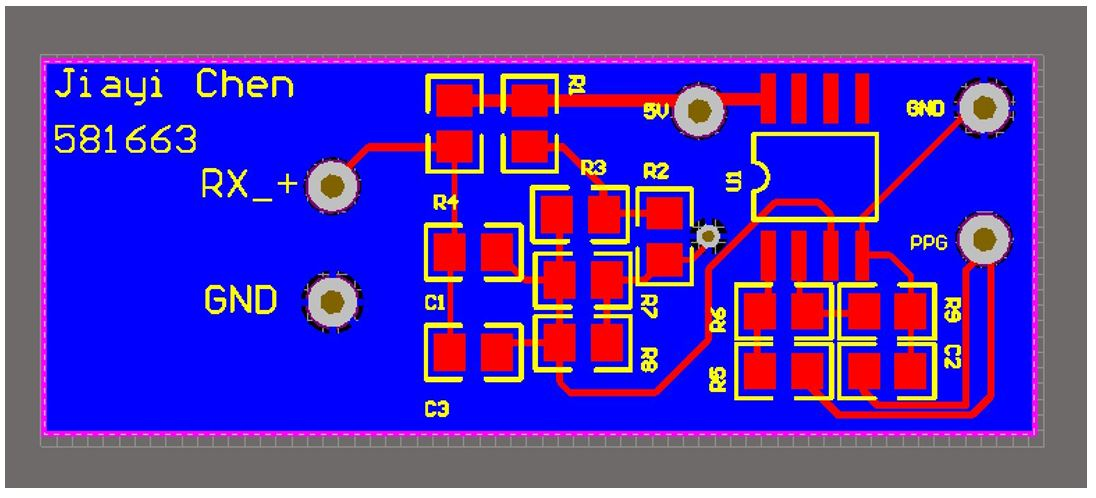
\includegraphics[width=\linewidth]{georgepic17.jpg}
	\caption{Receiver PCB for PPG}
\end{figure}